\section{Experimentation}

\subsection{Strategy Hierarchy}
The following Hierarchy shows how we could organize Team behavior across 5 layers, from high-level strategy down to low-level execution. Each layer builds on the one above it, enabling modular, scalable control.

\begin{figure}[h]
    \centering
    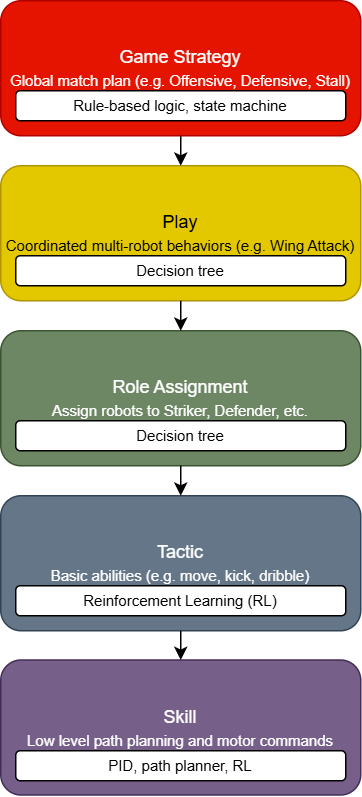
\includegraphics[width=0.8\linewidth]{../StrategyHierarchy.png}
    \caption{Hierarchical team behavior structure}
    \label{fig:strategy_hierarchy}
\end{figure}

\subsubsection{Game Strategy}
The top-layer defines the overall team behavior based on the given game state.
If we take Rule-based logic for example, we could look at time left to play and score.
Then if we are winning and the time is lower than a specified threshold, we could set the Strategy to Stall. This will then provide high-level context for all other decisions made below.

\subsubsection{Play}
The play layer selects coordinated maneuvers such as setting up a wing attack or forming a defensive wall. Selecting plays could be done by a decision tree based on factors like ball position, team formation, and opponent layout. Each play then sets constraints or goals for roles and tactics.

\subsubsection{Role Assignment}
This layer will dynamically assign robots to specific roles (e.g. striker, defender, goalie) based on their position, proximity to the ball, or other factors.
Optimization algorithms such as Hungarian matching have been used with great success.

\subsubsection{Tactic}
The tactic layer defines what action a robot should take in its current role.
This could be whether the robot should pass, dribble, shoot, or intercept.
This layer's decisions are highly context-sensitive and reinforcement learning is a good choice.

\subsubsection{Skill}
The skill layer handles the low-level physical execution of actions.
This could be moving to a position, kicking (how hard) or dribbling. Commonly used control methods are PID and path planning, but reinforcement learning can also be used to improve fine motor control, adaptability, or performance in unpredictable situations.

\subsection{Training}
To prepare our agents for RoboCup SSL, we are currently exploring VMAS (Vectorized Multi-Agent Simulator) as our training environment. VMAS is a lightweight and very customizable simulator to prototype and train multi-agent behaviors. We can set up custom scenarios that simulate different game situations. We can then use it to train both the Tactic and Skill layer behaviors using RL algorithms. In each scenario, we define the agent's observations, actions, and reward signals to shape the behavior we want them to learn. VMAS also supports fast, parallelized simulation with GPU acceleration, which allows us to efficiently run many environments at once. At this stage, we are still experimenting with different training approaches. The goal is to eventually transfer the trained policies to a more realistic simulator like grSim, where we can evaluate their performance in a full game setting.

\subsection{Agent Architecture: Single vs Multi-Agent}

At this stage, we are still exploring whether to model our AI system as a single-agent or a multi-agent architecture.

A \textbf{single-agent} approach would involve one central controller that receives the entire field state and outputs coordinated actions for all robots. This method simplifies coordination and is often easier to implement and train.

A \textbf{multi-agent} approach would assign each robot its own agent, possibly with limited field knowledge. This approach is more realistic and can model decentralized behavior, but introduces complexity in coordination and learning stability.

Our initial focus will likely lean toward the single-agent model to reduce complexity during development. However, we may transition to or experiment with a multi-agent setup depending on performance and scalability needs.
